\chapter{相关工作介绍}

\section{人类感光系统原理}
由于近年来蓬勃发展的神经形态视觉传感器追根溯源是受到了人类感光系统的启发,所以有必要讲解一下人类感光系统的原理,并随后分析这种原理如何被创造性地抽象化,利用和改进,以表现出和传统曝光相机在采样机制和数据结构上迥然不同的特点和成像高动态范围的优势。
\subsection{人类感光系统}
人类感光系统是多种细胞组成不同生理结构的有机结合,其核心为视网膜。如图\ref{fig:human_eye}所示,视网膜是一个由多种细胞组成的结构,是位于人眼眼球内侧的高度复杂的精细感光结构。从外层到内层分布着光感受器细胞外段层,包含视锥细胞和视杆细胞的外核层,外网状层,包含水平细胞和双极细胞的内核层,内网状层和向神经中枢传递神经信号的神经节细胞。正因为这些细胞的层次化有序排列,才能使得人眼拥有高分辨率,高动态范围的特性。这为神经形态视觉传感器提供结构和功能上的借鉴。

视网膜感光层的核心是视锥细胞和视杆细胞,它们将光信号转变为人脑可接受处理的电信号。视锥细胞对强光敏感,负责颜色识别,在中央凹区域尤为密集,也恰好是光线入眼的直接接受区域。视杆细胞对弱光敏感,负责照度识别,广泛分布在视网膜外围,构成全眼照度识别的基础。双极细胞处于更深层,接受上述两种细胞反馈的信号,根据光感受野的区域分成“开”、“关”两种形态。水平细胞横亘在外网状层,负责信息之间的传递,调节整体亮度并强化画面视觉边缘。

上述的人眼成像原理,为神经形态视觉传感器的研发提供了理论基础和灵感来源。通过对各种细胞的功能抽象和电子元件功能替代,我们可以设计出具有不同特性和优势的神经形态视觉传感器。
\begin{figure}[ht]
  \centering
  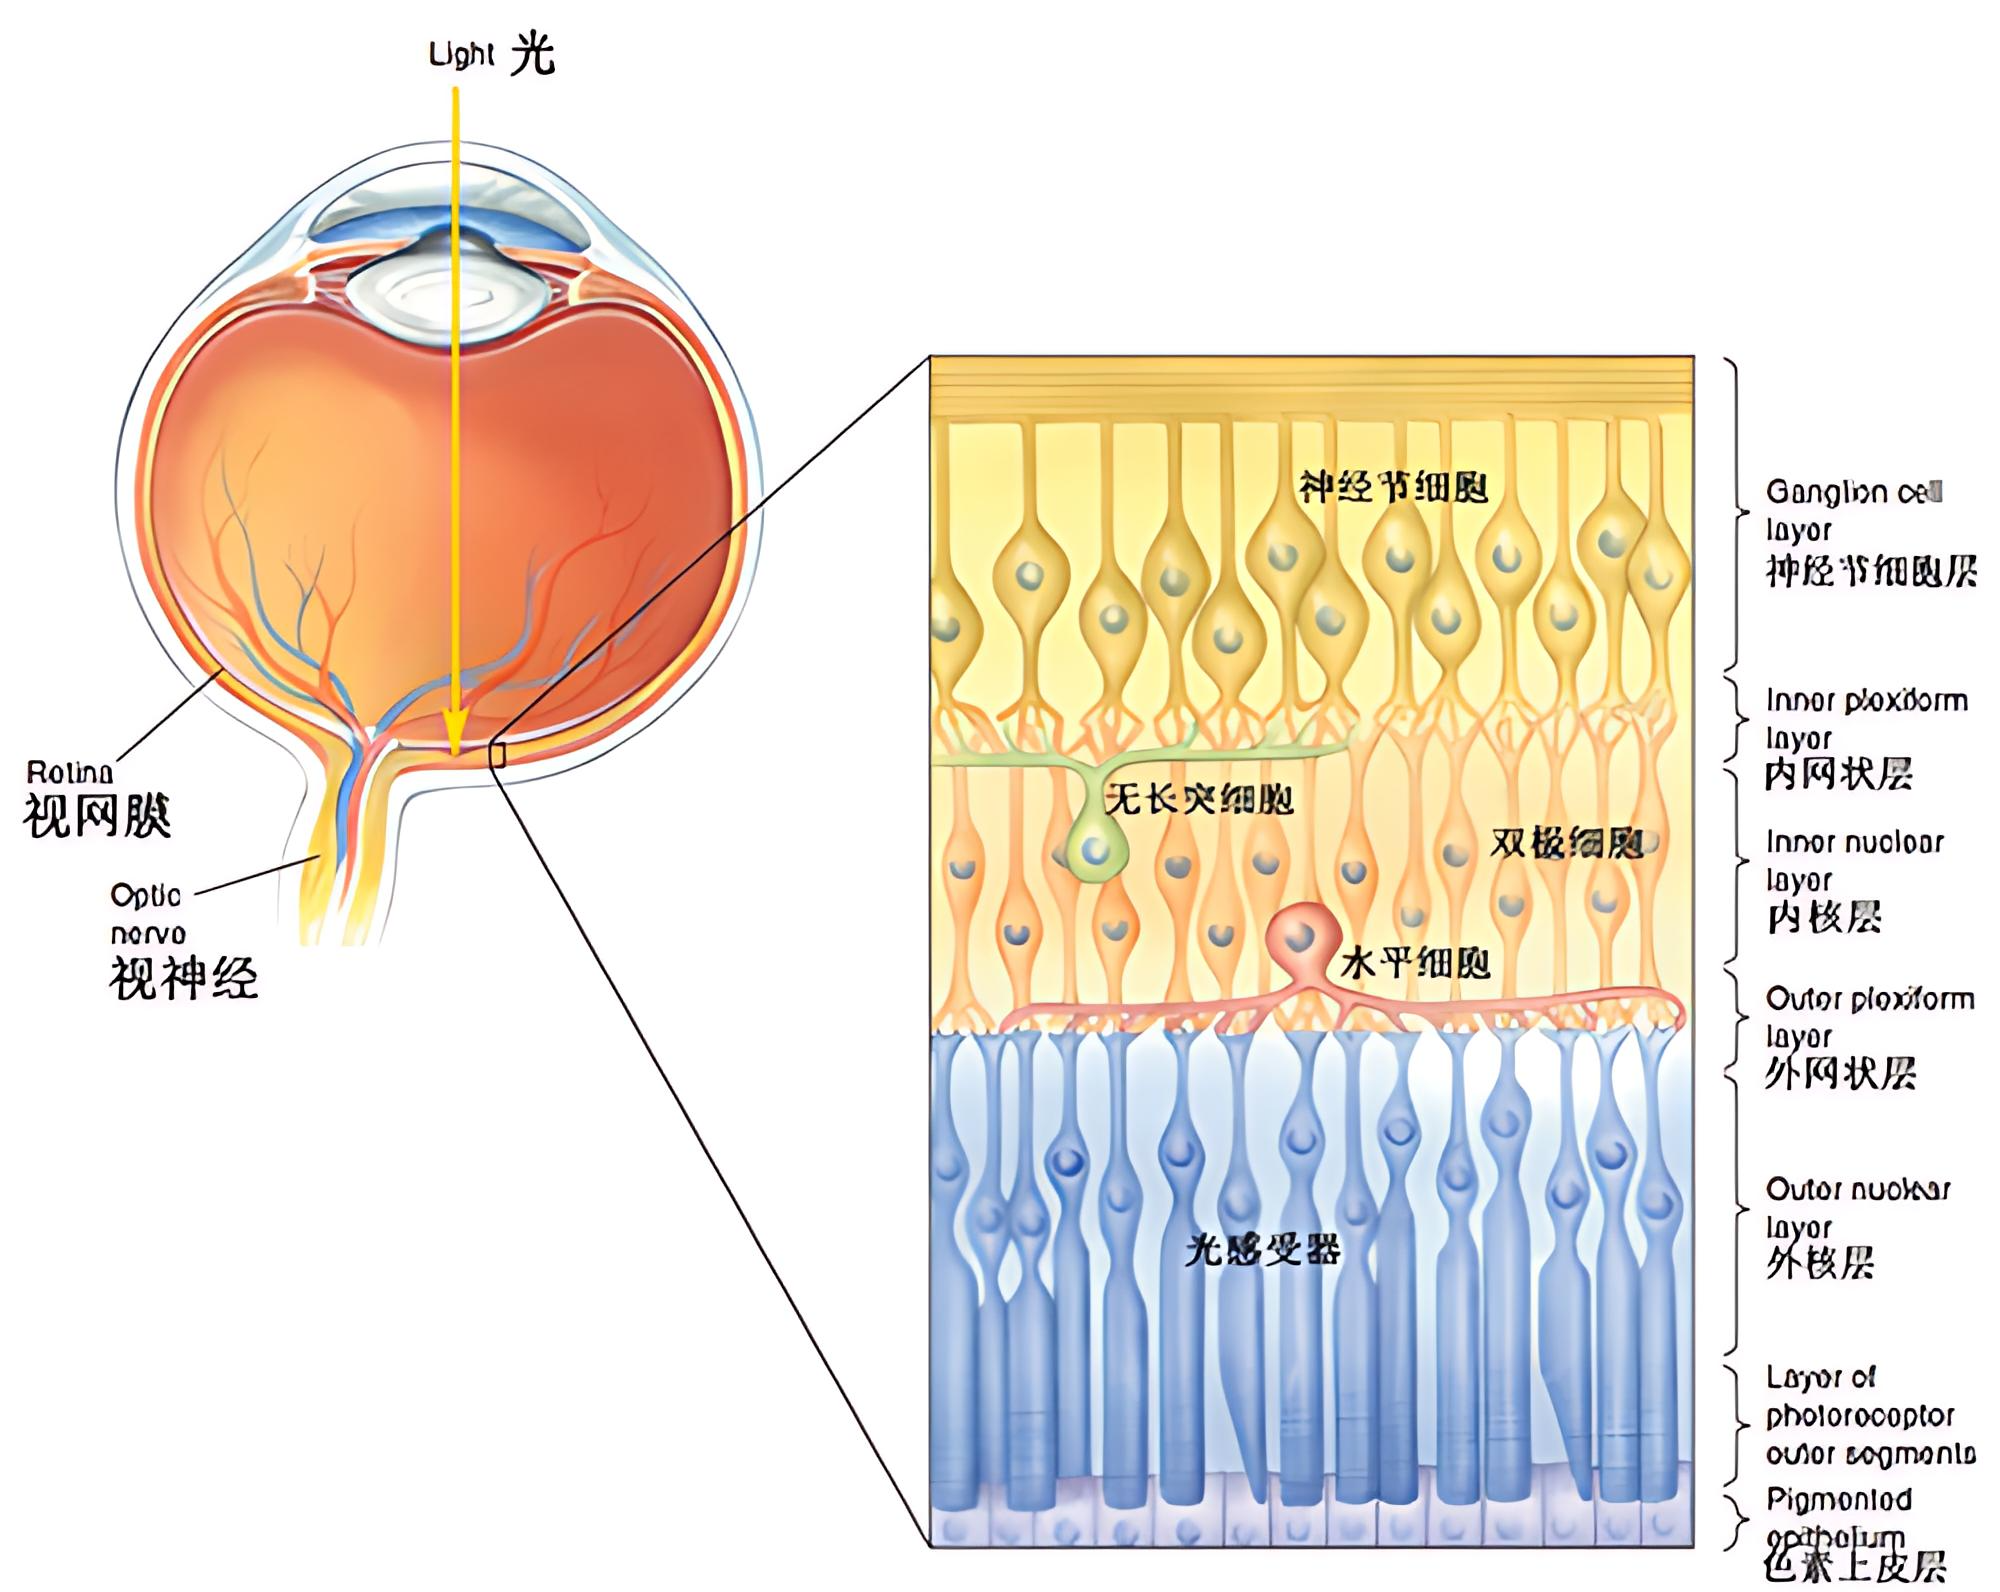
\includegraphics[width=\textwidth]{human_eye.png}
  \caption{人眼及其视网膜结构示意图}
  \label{fig:human_eye}
\end{figure}


\subsection{上述系统对脉冲相机的启发}
来自北京大学的Huang教授及其团队于2018年提出了仿视网膜中央凹采样模型(Fovea like Sampling Model,FSM)\cite{7923720}。此模型借鉴了上述人眼成像机制中视网膜中央凹的感知结构,突出其光敏优势,通过脉冲发放频率和脉冲宽度对光强进行积分,且由于自然界中光强客观存在,脉冲必定发放,通过人为或自适应设定脉冲发放阈值调节“光敏度”保持合理的脉冲密度,籍此避免了传统曝光相机在过暗和过亮情况下无法记录信息的问题。Huang教授及其团队进一步具象化上述原理,自主研发脉冲相机(Spike Camera),采用脉冲序列\cite{dong2018spike}形式传输数据,即高速脉冲帧。随后该团队在时间分辨率和空间分辨率上对硬件开展进一步的提升。表列出了两代Spike Camera的各项详细参数。

\begin{table}
  \centering
  \caption{Spike Camera的各项详细参数}
  \label{tab:spike_camera_parameter}
  \begin{tabular}{ccc}
    \toprule
    Spike Camera                & -Gen1\cite{dong2018spike} & -Gen3\cite{Huang_Tiejun110} \\
    \midrule
    年份                          & 2018                      & 2020                        \\
    空间分辨率(像素数)                  & 400\times250              & 1000\times1000              \\
    时间分辨率($\upmu$s)             & 50                        & 25                          \\
    动态范围(dB)                    & >110                      & >110                        \\
    最大数据通量(eps)                 & 2G                        & 40G                         \\
    芯片尺寸(mm\textsuperscript{2}) & 10\times6                 & 20\times20                  \\
    像素尺寸(平方毫米)                  & 20\times20                & 17\times17                  \\
    芯片制造工艺(nm)                  & 110                       & 110                         \\
    芯片工作电压(V)                   & 12                        & 12                          \\
    填充系数                        & 13.75\%                   & 13.75\%                     \\
    芯片功耗(mW)                    & 370                       & 3000                        \\
    数据接口                        & USB3.0                    & USB3.0                      \\
    \bottomrule
  \end{tabular}
\end{table}

\section{脉冲相机工作原理}

\begin{figure}[ht]
  \centering
  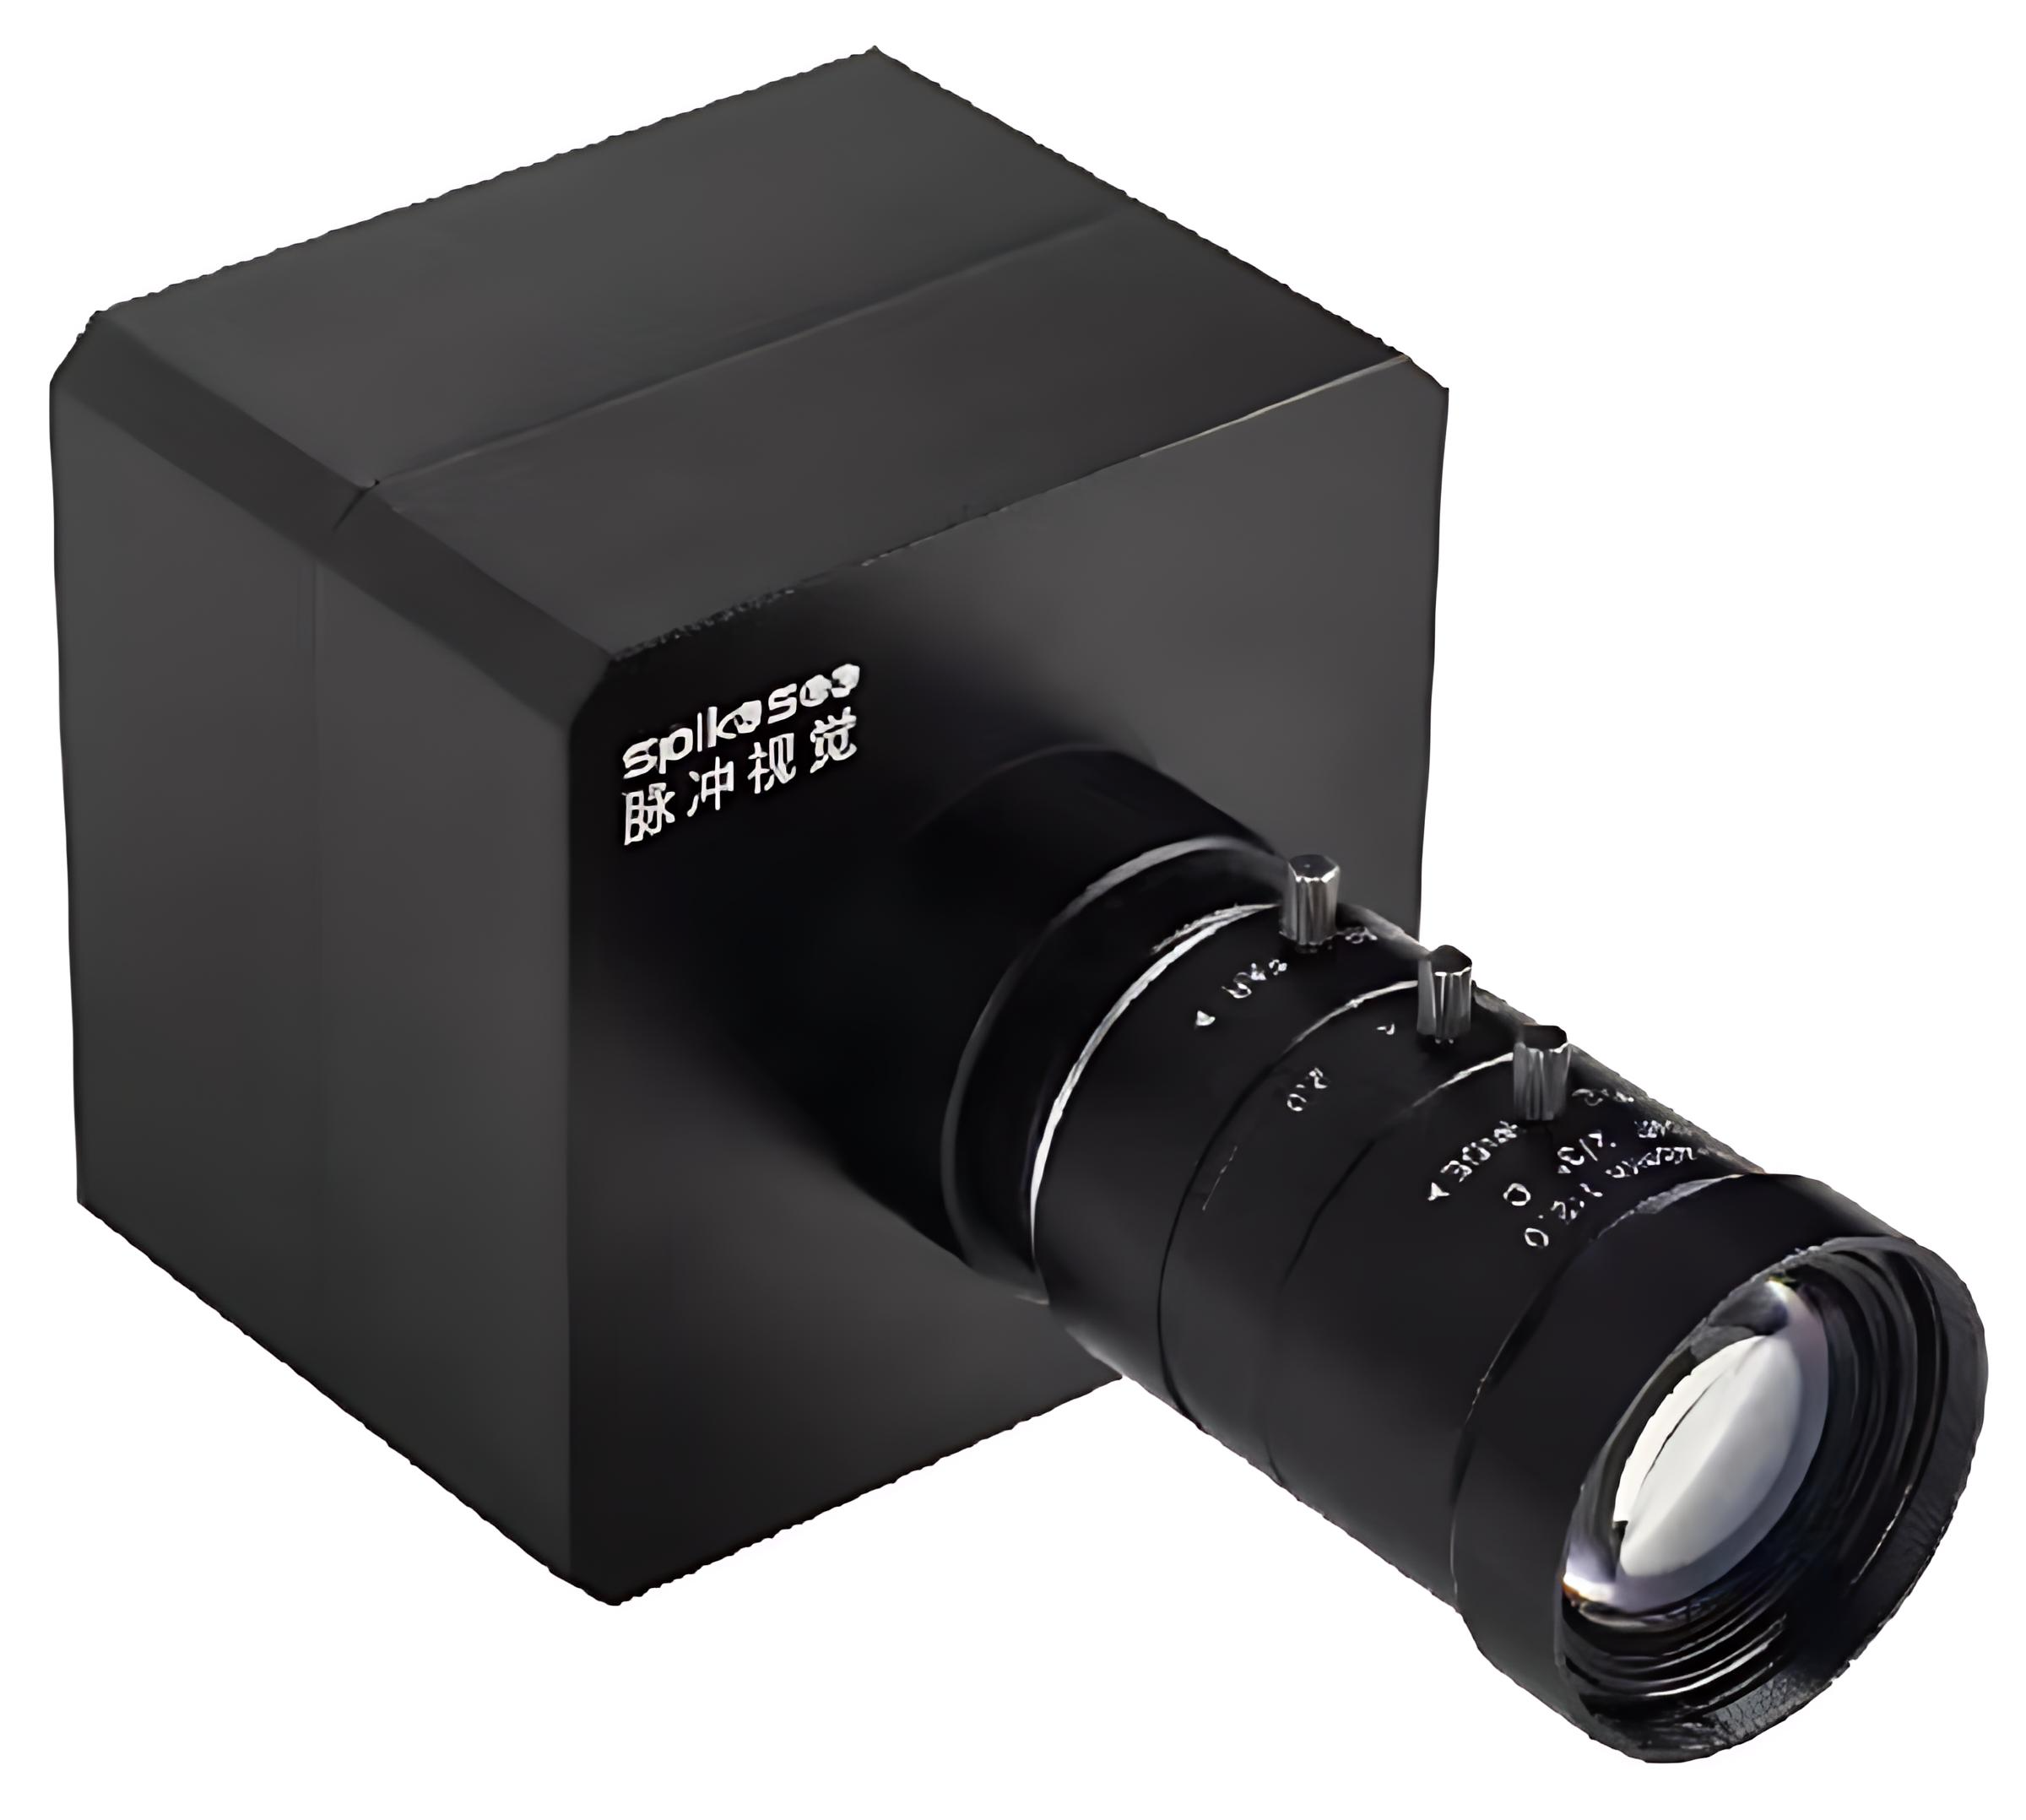
\includegraphics[width=\textwidth]{spike_camera_fig_clear.png}
  \caption{脉冲相机Gen1实例示意图}
  \label{fig:spike_camera_working_principle}
\end{figure}


脉冲相机的成像原理模拟视网膜中央凹区域神经元发放脉冲的原理,每一个像素点均由独立的电路结构构成,包含光感受器,自复位电路和脉冲读出电路,分别对应着脉冲信号产生的三个步骤——积分、复位和读出。在积分阶段感光部分的光电二极管持续吸收光子,使与其并联的电容上积累的电荷减少,电压降低。当电容上的电压降低至设定阈值$V_{th}$时比较器产生反转信号并驱动自复位电路生成复位信号复原光电二极管,使之复原到重新从零积累光子的状态,即新的积分阶段。当新的时钟信号来临时,自复位电路的信号被读出电路读取,且该信号被清除,重新进入复位前的阶段。而整个电路中可调节的参数为阈值电压和时钟频率。前者决定了单个脉冲所代表的光子数量,后者决定了芯片的最大脉冲发放频率,即芯片的时间分辨率。用数学公式表述上述过程如下。
\begin{equation}
  \label{eq:4}
  \frac{1}{C} \int_{t}^{t+\Delta t} I_s dt \geq V_{th}
\end{equation}

其中,$V_{th} = V_{dd} - V_{ref}$为设定电压阈值,$C$为电容,$I_s$为光电流强度,$\delta t$为积分时间,值得注意的是积分时间可以超过一个时钟周期,这对应着在环境光强过暗时可能需要多个时间周期才能积累到一个脉冲。由上述原理可推知下述理想情况下(忽略噪声,场景亮度稳定,电容无电荷泄露情况)单位时间内脉冲发放数量即脉冲频率的计算公式
\begin{equation}
  \label{eq:5}
  f_s = \frac{I_s}{CV_{th}}
\end{equation}
在一定时间$T_{given}$内,单个像素在理想情况下发放的脉冲数量$N_{s}$如下
\begin{equation}
  \label{eq:6}
  N_{s} = T_{given} f_s = \frac{T_{given} I_s}{CV_{th}}
\end{equation}

由此可知一定时间内发放脉冲的数量和场景光强成正比。


脉冲相机每个像素独立吸收转换光子,互不干扰。假设将脉冲相机感知光强和光电转换过程定义为A,场景光强定义为I,则脉冲序列的生成过程可以被表示为:
\begin{equation}
  \label{eq:1}
  S=R(A(I)+\mathcal{N})
\end{equation}
其中S代表在场景光强I的条件下产生的脉冲序列,R是脉冲序列的读出过程,$\mathcal{N}$是这个过程之中所有噪声之和。在理想情况下$\mathcal{N}$=0,S作为光强的真实表示。而在现实情况中,热噪声,散粒噪声,读出噪声等噪声之和由$\mathcal{N}$表示,对图像质量带来挑战。

在高速运动物体感知过程中,物体和相机的相对运动对成像的影响不可忽视,在极端情况下,超高速物体的像可以在一个时间步内移动超过一个像素,这就会带来可直接观察到的模糊。公式\ref{eq:1}可进一步被表示为:
\begin{equation}
  \label{eq:2}
  S_{t_{i-1} \rightarrow t_{i}}=R(M_{t_{i-1} \rightarrow t_{i}}A(I_{t_{i-1} \rightarrow t_{i}})+\mathcal{N})
\end{equation}
其中$M_{t_{i-1} \rightarrow t_{i}}$代表在时间$t_{i-1}$到时间$t_{i}$物体和相机高速运动的表示矩阵。由于脉冲相机时域采样分辨率较高,所以当相对运动相对较慢时,$M_{t_{i-1} \rightarrow t_{i}}$近似为单位矩阵。

脉冲视觉重建任务的目标是从一定长度的脉冲序列S之中重建原始清晰图像Y。将重建模型表示为$\mathcal{F}$并采用监督训练神经网络的方式实现,则问题的实现转变为以下表述方式:
\begin{equation}
  \label{eq:3}
  \hat{\theta} = \mathop{\arg\min}\limits_{\theta} \mathcal{L}(\mathcal{F}(\mathcal{T}(S),Y) + \lambda \phi(\theta))
\end{equation}
其中$\theta$和$\mathcal{L}$各自是模型$\mathcal{F}$的优化参数和损失函数,$\mathcal{T}$是脉冲序列的表征转换矩阵,$\phi$是正则化项,$\lambda$是正则化系数。

对于相机而言,成像的动态范围是其重要参数之一,决定了其能够测量的最高/低亮度的比值。根据动态范围计算公式
\begin{equation}
  \label{eq:7}
  DR = 20 \log_{10} \frac{L^{max}}{L^{min}}
\end{equation}

其中$L_{max}$和$L_{min}$分别为相机能够测量的最高亮度和最低亮度,$DR$(Dynamic Range)为动态范围。将其带入脉冲相机中得到脉冲相机动态范围计算公式:
\begin{equation}
  \label{eq:8}
  DR = 20 \log_{10} \frac{N^{max}_s}{N^{min}_s}
\end{equation}
其中$N^{max}_s$为一定时间内发射的脉冲数量的最大值,对应着最大可处理的场景光强,$N^{min}_s$为一定时间内发射的脉冲数量的最小值,对应着最小可处理的场景光强。这里采用脉冲数量进行计算,隐含着脉冲相机动态范围和接受光子的时间相关。在前述理想条件下,公式为无偏差估计,但在实际情况中,由于光子以Poisson分布随机发放,元件制成过程中的内在缺陷,电路读出过程中的读出噪声,电路运行时生热产生的热噪声,电路内部暗电流等都会影响测得脉冲。特别是由于暗电流的存在,在光强为零的条件下经过特定时间也可以产生脉冲。在光强较弱的条件下,暗电流的存在可能会导致信噪比受到较大影响,且这种影响是潜藏在脉冲内部的,不可被直接分开。

按照表\ref{tab:spike_camera_parameter}所示,采用Gen1版本相机进行数据计算,在40kHz的时钟频率下,时间窗口为1s时动态范围约为92dB,而要达到表中的大于110dB的动态范围,则时间窗口不小于7.9s。


\section{压缩感知图像重建算法研究现状}
\subsection{压缩感知理论发展概述}

\begin{figure}[ht]
  \centering
  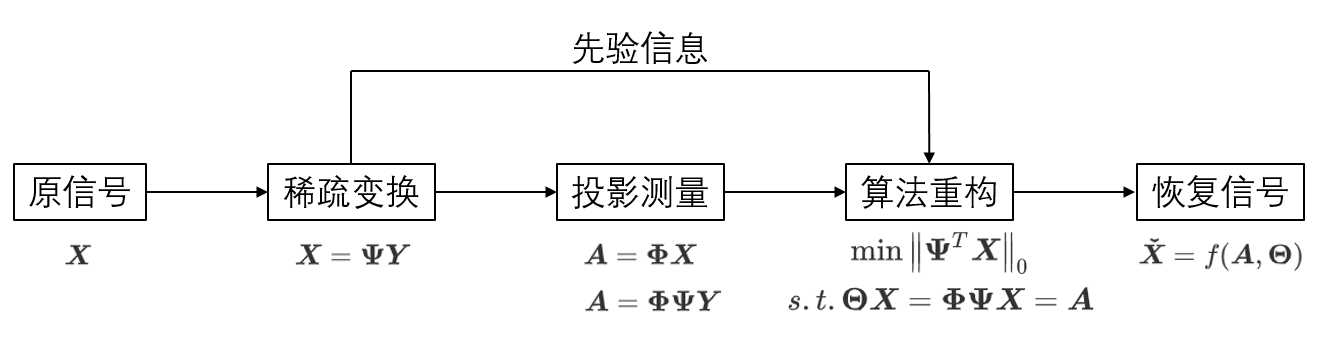
\includegraphics[width=\textwidth]{cs_principle.png}
  \caption{压缩感知框架}

\end{figure}
得益于21世纪以来计算机硬件条件的大幅提升和先进的机器学习算法的快速发展,计算机视觉的现实应用日益蓬勃,其解决问题的思路是:
\begin{enumerate}
  \item 获取各种形式(特定视角,特定数量,特定环境条件,特定设备,特定数据格式等)的目标任务涉及对象的视觉信息
  \item 对上述视觉信息进行初步处理(数据对齐,裁剪,增广等),形成所需的具备特定特点的数据集
  \item 利用对应算法组合对数据集进行运算并得到特定结果
  \item 将得到的最优算法在实际场景下检验有效性和鲁棒性
\end{enumerate}


但由于现实环境的时间空间充满不可量化的无穷变化,第一步为解决特定问题而准备的数据规模在不断膨胀,如果不加以处理很可能会超出计算机硬件的处理能力,导致算法无法收敛。这就要求科研工作者在数据数量和数据质量之间做出权衡。应运而生的,数据压缩感知算法在2006年被David L. Donoho等人首次提出\citep{David_compress,An_Introduction_To_Compressive_Sampling,Extensions_of_compressed_sensing},其主要思想是突破奈奎斯特采样定理,解决传统数据必须先采样后压缩的弊端,通过在采样时即采用稀疏矩阵对原数据进行稀疏化,使得原信号或信号在某个变换域上稀疏,用向量的语言表述则是使向量中尽可能多的元素为零从而减少数据量。然后通过采样矩阵将原高维信号投影到低维空间。压缩感知相较于传统先采样后压缩的方式而言, 可以通过稀疏矩阵和采样矩阵结合为压缩矩阵,来实现采样和压缩同时进行。这样既降低硬件设备的要求, 又节约数据在传输和运算过程中的所需带宽。这是其在数据压缩层面的主要贡献。而将其应用到图像重建上,则实现了图像信息的投射变换和降维,寻找图像分解的变换基,从而在变换中将内在特征不同的图像信息和噪声信息区别开来,离散余弦变换变换(discrete cosine transform, DCT)\cite{DCT},快速傅里叶变换等将图片从空间域变换至频域的算法,通过删除高频信息实现了图像本征信息的保留和压缩。这是其在图像去噪,去模糊等方向上的贡献。如图\ref{fig:FFT_IMAGE}所示,经过快速傅里叶变换后图像整体视觉信息大部得到保留,图像的浅色部分代表的高频信息的损失只产生了可以被人眼接受并在识别允许范围内的噪声。这充分体现了图片信息的冗余性。


\begin{figure}[htbp]
  \centering
  % 第一行图片
  \begin{subfigure}[b]{0.45\textwidth}
    \centering
    
\includegraphics[width=\textwidth]{original_image_skimage.jpg}
    \caption{原始图像}
    \label{fig:sub1}
  \end{subfigure}
  \hfill
  \begin{subfigure}[b]{0.45\textwidth}
    \centering
    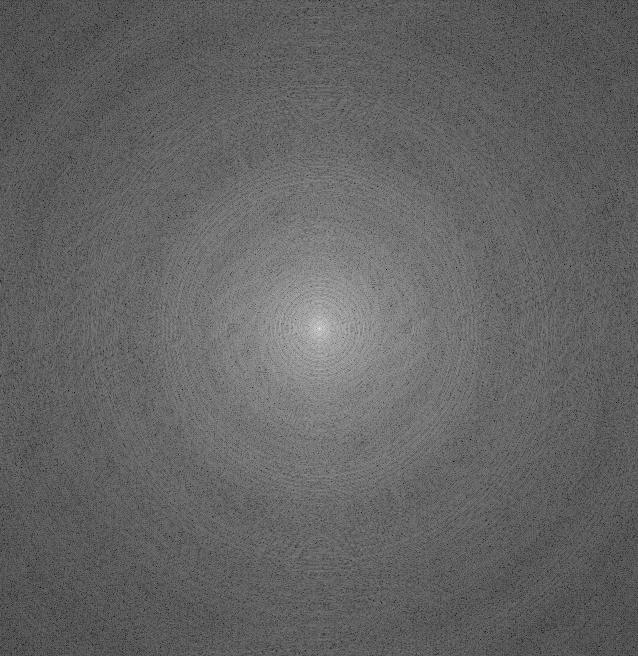
\includegraphics[width=\textwidth]{fourier_transform_skimage.jpg}
    \caption{FFT转换后的频谱}
    \label{fig:sub2}
  \end{subfigure}

  % 第二行图片
  \vskip\baselineskip
  \begin{subfigure}[b]{0.45\textwidth}
    \centering
    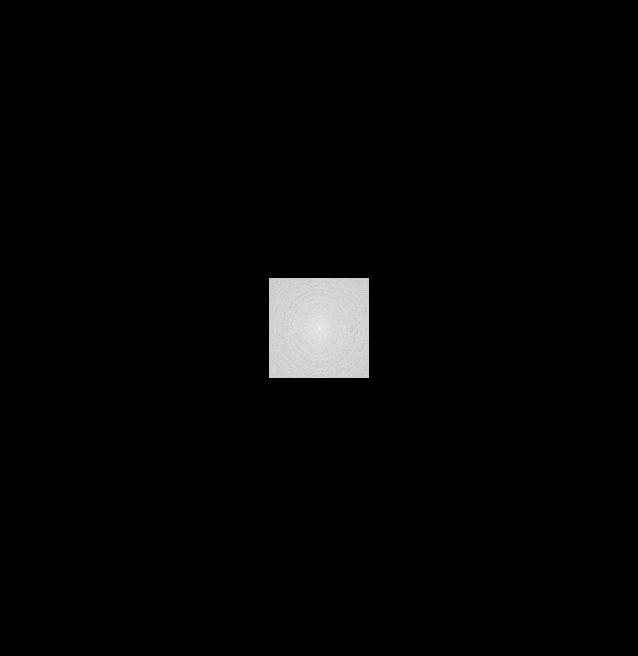
\includegraphics[width=\textwidth]{filtered_spectrum_skimage.jpg}
    \caption{滤去高频后的频谱}
    \label{fig:sub3}
  \end{subfigure}
  \hfill
  \begin{subfigure}[b]{0.45\textwidth}
    \centering
    
\includegraphics[width=\textwidth]{inverse_fourier_transform_skimage.jpg}
    \caption{过滤后逆变换所得图像}
    \label{fig:sub4}
  \end{subfigure}
  \caption{将原始图像通过快速傅里叶变换,高频率波谱去除,再进行逆傅里叶变换得到的图像}
  \label{fig:FFT_IMAGE}
\end{figure}

\subsection{基于先验知识的传统压缩感知重建方法}

传统压缩感知算法主要有基追踪算法(BP)、内点法(IPM)、梯度投影
法(GPSR)  、 迭代阈值法(ISTA) 和交替方向
乘子法(ADMM)  等. 常见的贪婪算法有匹配追
踪算法(MP) 、 正交匹配追踪算法(OMP)  和压
缩采样匹配追踪算法(CoSaMP) 。其中对比详见表\ref{tab:reconstruction_methods}。


\begin{table}[htbp]
  \centering
  \caption{传统基于先验知识的压缩感知重建方法及典型的实现算法}
  \label{tab:reconstruction_methods}
  \resizebox{\textwidth}{!}{
    \begin{tabular}{cm{3cm}m{3cm}c} % 使用 m{宽度} 使内容垂直居中,删除类别列
      \toprule
      方法                                   & 算法                               & 年份   & 特点分析                                        \\
      \midrule
      \multirow{4}{*}{\centering 凸松弛方法}    & BP\cite{chen1998atomic}          & 1998 & \multirow{4}{*}{\centering 有理论保证,计算复杂度高}    \\
                                           & IPM\cite{monteiro1998interior}   & 1998 &                                             \\
                                           & GPSR\cite{recknagel2011gradient} & 2011 &                                             \\
                                           & ISTA\cite{beck2009fast}          & 2009 &                                             \\
      \cline{2-4}
      \multirow{3}{*}{\centering 贪婪匹配追踪方法} & MP\cite{mallat1993matching}      & 1993 & \multirow{3}{*}{\centering 无理论保证,实现简单,速度较快} \\
                                           & OMP\cite{pati1993orthogonal}     & 1993 &                                             \\
                                           & CoSaMP\cite{needell2009cosamp}   & 2009 &                                             \\
      \cline{2-4}
      \multirow{2}{*}{\centering 贝叶斯类方法}   & BCS\cite{baraniuk2008bayesian}   & 2008 & \multirow{2}{*}{\centering 利用参数的先验信息,有鲁棒性}  \\
                                           & BCS - LP\cite{rauhut2010sparse}  & 2010 &                                             \\
      \bottomrule
    \end{tabular}
  }
\end{table}

凸松弛方法上述已经说明,核心思想是将最小 l0 范数问题在一定条
件下等价地转化为求解最小 l1 范数问题。贪婪匹配追踪方法是在每次迭代时,通过计算残差与原子的内积,选择局部最优原子,再计算该原子系数,逐步近似原始信号。这种方法并不能够确保得到最优信号。而贝叶斯类方法由先验知识得到信号的先验概率密度分布函数,然后用最大后验概率估计,对重构值的误差范围进行估计,进而重构出原始信号。贝叶斯方法考虑信号观测时引入的噪声,通过噪声的先验概率密度分布和最大后验概率估计,得到噪声的最大估计值。在做先验概率密度分布时,通常使用拉普拉斯分布、伽马分布等概率分布函数,或者使用相关向量机算法做先验分析,再用高斯分布模拟噪声环境。贝叶斯类重建方法的重建精度和时间复杂度介于凸松弛方法和贪婪匹配追踪方法之间,因其加入了噪声的重建,比贪婪匹配追踪算法的重建结果更优,比凸松弛方法具有更低的计算复杂度。

基于先验知识的重建方法优点在于它们基于可解释的先验知识并且便于理解,而且当基于 l0 范数最小的重建问题转换并建模为凸优化问题求解时有理论收敛保证。然而这些使用信号先验知识的方法应用于实时图像压缩感知问题时存在运算速度过慢,未利用信号本身的特征的问题。

\subsection{基于深度学习的压缩感知重建方法}
近年来研究人员意识到大批量数据自身内部的数据特征未被合理利用的现实和这个现实可能对压缩感知效果的巨大提升,采用数据驱动的深度学习算法,以神经网络的形式取代了原有的先验知识模型。在信号重建方面,深度学习方法具有强大的非线性映射能力。传统的压缩感知重建算法如上述的凸优化或贪婪算法,计算复杂度高且在复杂信号情况下重建效果不佳。而深度学习通过构建深度神经网络,如卷积神经网络(CNN)和循环神经网络(RNN),可以自动学习信号的特征和分布,从而实现高效准确的信号重建。例如,在图像压缩感知中,CNN 能够捕捉图像的局部特征和纹理信息,通过端到端的训练,直接从压缩测量值中恢复出高质量的图像。

\begin{figure}[ht]
  \centering
  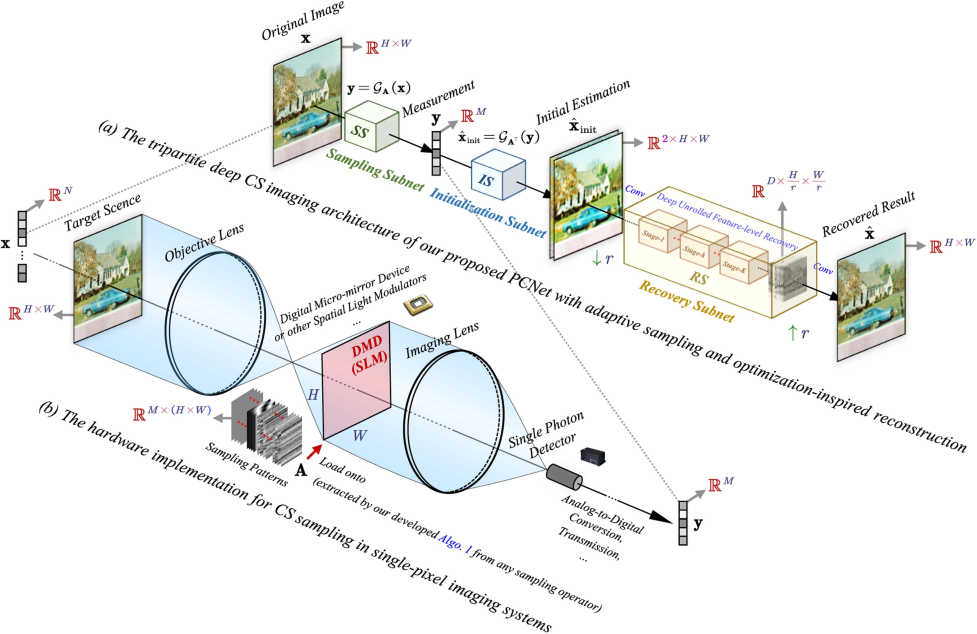
\includegraphics[width=\textwidth]{dnn_cs.png}
  \caption{深度神经网络用于压缩感知的整体结构和现实映射\cite{Practical_compact_deep_compressed_sensing}}
  \label{fig:dnn_cs}
\end{figure}

上图\ref{fig:dnn_cs}展示了深度神经网络在压缩感知中的范式。首先原始图片x经过采样子网得到观测值y,子网可以采取不同的采样方式,如随机采样、均匀采样、高斯采样等。然后将观测值y输入到初始化子网中,初步得到重建图像$\hat{x_{init}}$。这一步可以采用随机矩阵,但通过合理的设计和初始值的估计可以达到逼近原始图像的效果,节省网络收敛的时间。最后,通过重建网络的深度展开迭代,减小重建误差,最终得到该数据集训练出的网络和重建结果$\hat{x}$。对应到硬件设计上,通过(b)中所展示的不同微透镜阵列实现不同模式的采样矩阵,用M个单独的调制模式(每个模式对应于大小为 H × W 的矩阵行),以单独加载到特定的空间光调制器 (SLM) 上,实现单独采样。

近年来基于深度学习的压缩感知算法可以根据观测矩阵类型、是否可训练两个角度进行分类。详细分类根据\cite{Practical_compact_deep_compressed_sensing}见表:

% \begin{table}[htbp]
%   \centering
%   \caption{基于深度学习的压缩感知重建方法及典型的实现算法}
%   \label{tab:reconstruction_methods_deeplearning}
%   \resizebox{\textwidth}{!}{
%     \begin{tabular}{ccccccc}
%       \toprule
%       方法                                                  & 年份  & 传感网络类型             & 是否可训练 & 传感网络参数量  & 迭代算法        & 总参数量  \\
%       \midrule
%       ReconNet\cite{ReconNet}                             & 2016  & \multirow{5}{*}{块状对角高斯矩阵} & \multirow{5}{*}{否} & \multirow{5}{*}{0} & -               & 0.62      \\
%       ISTA-Net$^{+}$\cite{ISTA-Net}                       & 2018  &                                 &                   &                   & ISTA\cite{beck2009fast} & 0.34    \\
%       DPA-Net\cite{DPA-Net}                               & 2020  &                                 &                   &                   & -               & 9.31      \\
%       MAC-Net\cite{MAC-Net}                               & 2021  &                                 &                   &                   & -               & 6.12      \\
%       ISTA-Net$^{++}$\cite{ISTA-Net++}                    & 2019  &                                 &                   &                   & PGD\cite{PGD}   & 0.76      \\
%       \cline{1-2}\cline{5-7}
%       CSNet$^{+}$\cite{CSNET}                             & 2019  & \multirow{8}{*}{块状对角可学习矩阵} & \multirow{8}{*}{是} & 1.05          & -               & 1.46      \\
%       SCSNet\cite{SCSNET}                                 & 2020  &                                 &                   & 1.05          & -               & 1.64      \\
%       OPINE-Net$^{+}$\cite{OPINE-NET}                     & 2021  &                                 &                   & 1.19          & ISTA\cite{beck2009fast}            & 1.10      \\
%       AMP-Net\cite{AMP-NET}                               & 2021  &                                 &                   & 1.05          & AMP\cite{AMP}   & 1.71      \\
%       COAST\cite{COAST}                                   & 2021  &                                 &                   & 1.19          & PGD\cite{PGD}   & 1.60      \\
%       MADUN\cite{MADUN}                                   & 2021  &                                 &                   & 1.19          & PGD\cite{PGD}   & 3.60      \\
%       FSOINet\cite{FSOINET}                               & 2022  &                                 &                   & 1.05          & PGD\cite{PGD}   & 1.06      \\
%       CASNet\cite{CASNET}                                 & 2022  &                                 &                   & 1.05          & PGD\cite{PGD}   & 16.90     \\
%       \cline{1-2}\cline{5-7}
%       RK-CCSNet\cite{RK-CCSNet}                           & 2020  & \multirow{2}{*}{堆栈网络}     & \multirow{2}{*}{是} & 0.11          & -               & 0.74      \\
%       MR-CCSNet$^{+}$\cite{MR-CCSNet}                     & 2022  &                                 &                   & 0.04          & -               & 14.25     \\
%       \cline{1-2}\cline{5-7}
%       PCT\cite{Practical_compact_deep_compressed_sensing} & 2025  & COSO\cite{Practical_compact_deep_compressed_sensing}                 & 可                & 0.05          & PGD\cite{PGD}   & 0.82      \\
%       \bottomrule
%     \end{tabular}
%   }
% \end{table}

\begin{table}[htbp]
  \centering
  \caption{基于深度学习的压缩感知重建方法及典型的实现算法}
  \label{tab:reconstruction_methods_deeplearning}
  \resizebox{\textwidth}{!}{
    \begin{tabular}{ccccccc}
      \toprule
      方法                                                  & 年份  & 传感网络类型             & 是否可训练 & 传感网络参数量  & 迭代算法        & 总参数量  \\
      \midrule
      ReconNet                             & 2016  & \multirow{5}{*}{块状对角高斯矩阵} & \multirow{5}{*}{否} & \multirow{5}{*}{0} & -               & 0.62      \\
      ISTA-Net$^{+}$                       & 2018  &                                 &                   &                   & ISTA & 0.34    \\
      DPA-Net                               & 2020  &                                 &                   &                   & -               & 9.31      \\
      MAC-Net                               & 2021  &                                 &                   &                   & -               & 6.12      \\
      ISTA-Net$^{++}$                    & 2019  &                                 &                   &                   & PGD   & 0.76      \\
      \cline{1-2}\cline{5-7}
      CSNet$^{+}$                             & 2019  & \multirow{8}{*}{块状对角可学习矩阵} & \multirow{8}{*}{是} & 1.05          & -               & 1.46      \\
      SCSNet                                 & 2020  &                                 &                   & 1.05          & -               & 1.64      \\
      OPINE-Net$^{+}$                     & 2021  &                                 &                   & 1.19          & ISTA            & 1.10      \\
      AMP-Net                               & 2021  &                                 &                   & 1.05          & AMP   & 1.71      \\
      COAST                                   & 2021  &                                 &                   & 1.19          & PGD   & 1.60      \\
      MADUN                                   & 2021  &                                 &                   & 1.19          & PGD   & 3.60      \\
      FSOINet                               & 2022  &                                 &                   & 1.05          & PGD   & 1.06      \\
      CASNet                                 & 2022  &                                 &                   & 1.05          & PGD   & 16.90     \\
      \cline{1-2}\cline{5-7}
      RK-CCSNet                           & 2020  & \multirow{2}{*}{堆栈网络}     & \multirow{2}{*}{是} & 0.11          & -               & 0.74      \\
      MR-CCSNet$^{+}$                     & 2022  &                                 &                   & 0.04          & -               & 14.25     \\
      \cline{1-2}\cline{5-7}
      PCT                                 & 2025  & COSO                 & 可                & 0.05          & PGD   & 0.82      \\
      \bottomrule
    \end{tabular}
  }
\end{table}

